\chapter{网络层}\label{CN04}

\section{路由、转发、SDN与拥塞}\label{CN04-forwarding}

IP在不同链路技术之上提供统一的尽最大努力数据报服务。路由选择依据可达性、度量和策略形成路径信息；转发对当前分组查表选输出接口和下一跳。普通路由器处理到网络层，下一跳用新的链路格式封装；协议转换须有明确的转换功能。

\par\smallskip
{\fontsize{9.3}{12}\selectfont\setlength{\tabcolsep}{2.5pt}\setlength{\LTleft}{0pt}\setlength{\LTright}{0pt}
\begin{longtable}{@{}>{\raggedright\arraybackslash}p{\dimexpr0.26748\linewidth-2\tabcolsep\relax}>{\raggedright\arraybackslash}p{\dimexpr0.73252\linewidth-2\tabcolsep\relax}@{}}
\toprule
路由方式 & 性质 \\

\midrule\endfirsthead\toprule
路由方式 & 性质 \\

\midrule\endhead\bottomrule\endfoot
静态 & 人工配置，开销低，故障适应依赖维护 \\

动态 & 交换信息自动更新，有报文、计算和收敛成本 \\

层次 & 区域或AS内部掌握细节，对外汇总；减少信息量，可能牺牲全局最短路径 \\

\end{longtable}}
\par\smallskip

SDN逻辑分离控制平面与数据平面：控制器计算并下发规则，交换设备匹配流表执行转发、丢弃、改写或上送。逻辑集中可由多个物理控制器实现；已有匹配规则无需逐包询问控制器。北向接口连接应用与控制器，南向连接控制器与设备，OpenFlow是南向协议之一。流表可按入端口、MAC、IP、协议、端口匹配，含优先级、计数器和动作。

拥塞源于多个输入竞争共享资源，持续到达速率超过服务速率会积压、丢包；加缓存只能吸收部分突发，可能增加时延。流量控制保护接收端，拥塞控制保护网络承载。可采用准入、整形、调度、主动丢弃/标记和反馈减速。全双工每方向分别合计汇聚流量，与该方向容量比较。

\section{距离向量与链路状态算法}\label{CN04-routing-algorithms}

距离向量由邻居通告到各目的的距离：

\[D_x(d)=\min_{v\in N(x)}\{c(x,v)+D_v(d)\}.\]

先加本机到邻居代价，再比较候选；取最小者作为下一跳，同值按题意处理。坏消息可形成环路并计数到无穷，水平分割、毒性逆转和触发更新只能按各自条件缓解。

\par\medskip\Needspace{4\baselineskip}\noindent\hypertarget{CN04-E01}{}\label{CN04-E01}\textbf{例 4-1}\par\nobreak\smallskip

某网络中的所有路由器均采用距离向量路由算法。路由器E与邻居A、B、C、D的直接链路距离分别是8、10、12、6，收到的距离向量如下。E更新后到Net1～Net4的距离分别是（　）。

\par\smallskip
{\fontsize{9.3}{12}\selectfont\setlength{\tabcolsep}{2.5pt}\setlength{\LTleft}{0pt}\setlength{\LTright}{0pt}
\begin{longtable}{@{}>{\raggedright\arraybackslash}p{\dimexpr0.30817\linewidth-2\tabcolsep\relax}>{\raggedright\arraybackslash}p{\dimexpr0.34592\linewidth-2\tabcolsep\relax}>{\raggedright\arraybackslash}p{\dimexpr0.34592\linewidth-2\tabcolsep\relax}@{}}
\toprule
目的网络 & A、B的通告 & C、D的通告 \\

\midrule\endfirsthead\toprule
目的网络 & A、B的通告 & C、D的通告 \\

\midrule\endhead\bottomrule\endfoot
Net1 & 1，23 & 20，22 \\

Net2 & 12，35 & 30，28 \\

Net3 & 24，18 & 16，36 \\

Net4 & 36，30 & 8，24 \\

\end{longtable}}
\par\smallskip

A. 9，10，12，6　B. 9，10，28，20

C. 9，20，12，20　D. 9，20，28，20

链路状态流程：发现邻居和测量代价\ensuremath{\to}在规定范围洪泛本地链路状态\ensuremath{\to}建立拓扑数据库\ensuremath{\to}各自以本机为根运行最短路径算法。通告用序号和老化区分新旧。非负权Dijkstra每轮选暂定距离最小的未确定节点，确定后松弛相邻边，保存前驱并推出下一跳。

\section{IPv4首部与分片}\label{CN04-ipv4}

\begin{figure}[H]
\centering
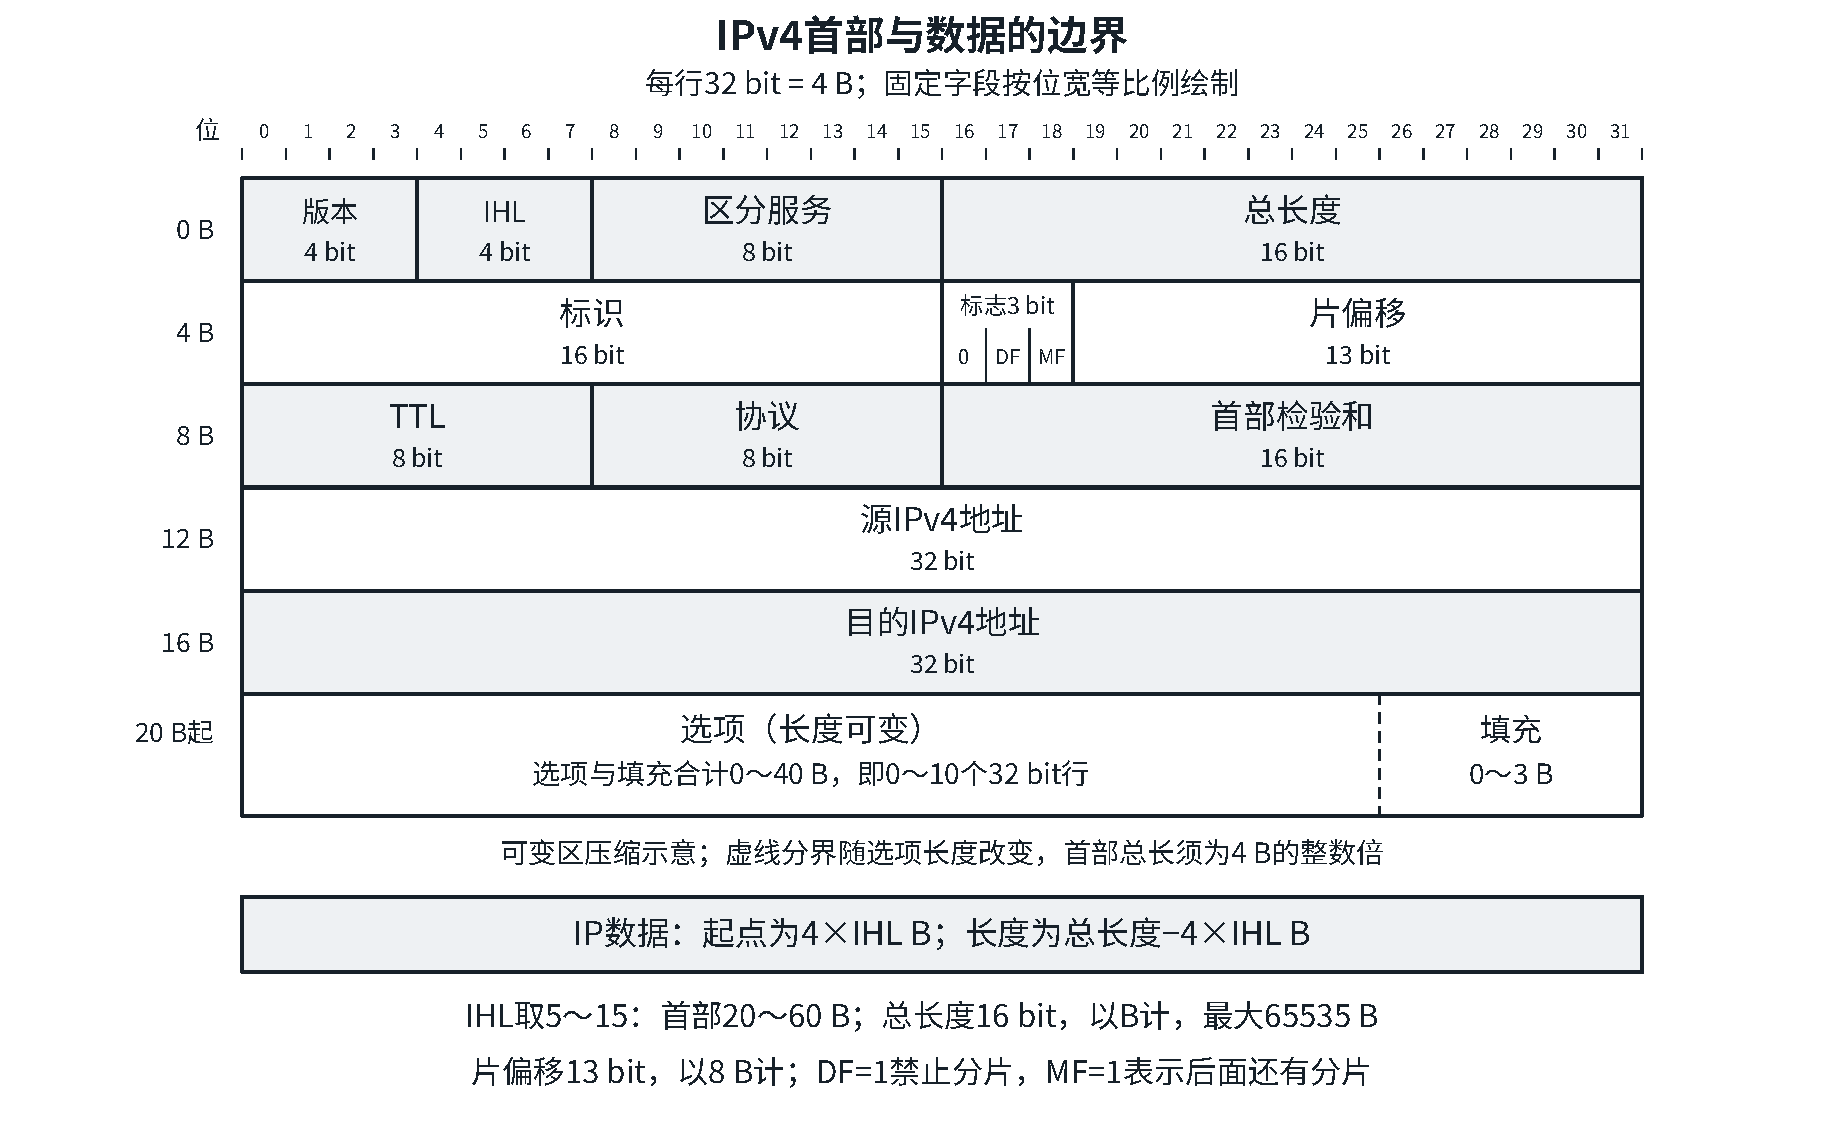
\includegraphics[width=\linewidth,height=108mm,keepaspectratio]{figures/CN16_ipv4_header.pdf}
\caption{IPv4固定首部20 B，可选部分另计}\label{cn-fig-ipv4-format}
\end{figure}

\par\smallskip
{\fontsize{9.3}{12}\selectfont\setlength{\tabcolsep}{2.5pt}\setlength{\LTleft}{0pt}\setlength{\LTright}{0pt}
\begin{longtable}{@{}>{\raggedright\arraybackslash}p{\dimexpr0.26494\linewidth-2\tabcolsep\relax}>{\raggedright\arraybackslash}p{\dimexpr0.21633\linewidth-2\tabcolsep\relax}>{\raggedright\arraybackslash}p{\dimexpr0.51873\linewidth-2\tabcolsep\relax}@{}}
\toprule
字段 & 位数 & 单位、含义与条件 \\

\midrule\endfirsthead\toprule
字段 & 位数 & 单位、含义与条件 \\

\midrule\endhead\bottomrule\endfoot
版本、IHL & 各4 & 版本4；首长\(H=4IHL\) B，IHL=5～15，首部20～60 B \\

区分服务 & 8 & 服务分类与拥塞标记 \\

总长度 & 16 & 首部与数据共计，B，最大65535 \\

标识 & 16 & 同一原数据报分片保持；重组还结合源、目的、协议 \\

标志 & 3 & 保留0；DF=1禁分片；MF=1原数据后面还有片 \\

片偏移 & 13 & 8 B单位，相对原始IP数据区起点 \\

TTL & 8 & 转发每跳减1，耗尽丢弃，条件允许时报告超时 \\

协议 & 8 & ICMP=1、TCP=6、UDP=17，用于网络层分用 \\

首部检验和 & 16 & 只覆盖IPv4首部，TTL或地址变化须更新 \\

源、目的地址 & 各32 & 标识源、目的IP接口 \\

\end{longtable}}
\par\smallskip

MTU约束完整IP分组。超MTU且DF=0可分片，每片有独立IP首部，目的主机重组；DF=1则丢弃并在允许时通知源端。非末片数据长度须为8 B整数倍，偏移不计任何IP首部。未分片为MF=0且偏移0，末片MF=0但偏移可非0。

首部固定\(H\)、出口MTU为\(M\)时，非末片最大数据量：

\[D_{max}=8\left\lfloor\frac{M-H}{8}\right\rfloor.\]

先算原数据长``总长减原首长''，列各片原数据区间，再填总长、偏移和MF。再次分片仍用原数据坐标，原片MF=1时，其最后子片也为MF=1。分片只切IP数据，不给每片再添TCP/UDP首部。

\par\medskip\Needspace{4\baselineskip}\noindent\hypertarget{CN04-E02}{}\label{CN04-E02}\textbf{例 4-2}\par\nobreak\smallskip

若路由器向MTU=800 B的链路转发一个总长度为1580 B的IP数据报（首部长度为20 B）时进行了分片，且每个分片尽可能大，则第2个分片的总长度字段和MF标志位的值分别是（　）。

A. 796，0　B. 796，1　C. 800，0　D. 800，1

\section{CIDR、特殊地址与子网划分}\label{CN04-addresses}

IPv4按32位处理。地址\(A\)、掩码\(M\)、前缀\(p\)：网络地址\(N=A\mathbin{\&}M\)；地址块大小\(2^{32-p}\)；广播地址\(N+2^{32-p}-1\)。普通多址子网主机位\(h\)，可分配\(2^h-2\)，网关接口也占地址。点对点\texttt{/\allowbreak{}31}、主机路由\texttt{/\allowbreak{}32}按特殊用途处理。

\par\smallskip
\begin{wideblock}
{\fontsize{9.3}{12}\selectfont\setlength{\tabcolsep}{2.5pt}\setlength{\LTleft}{0pt}\setlength{\LTright}{0pt}
\begin{longtable}{@{}>{\raggedright\arraybackslash}p{\dimexpr0.40552\linewidth-2\tabcolsep\relax}>{\raggedright\arraybackslash}p{\dimexpr0.59448\linewidth-2\tabcolsep\relax}@{}}
\toprule
地址或类别 & 用途 \\

\midrule\endfirsthead\toprule
地址或类别 & 用途 \\

\midrule\endhead\bottomrule\endfoot
\texttt{0.0.0.0} & 未获地址时可作本机源地址 \\

\texttt{255.255.255.255} & 本地受限广播，路由器不转发 \\

\texttt{127.0.0.0/8} & 回环，不作外部链路普通地址 \\

主机位全1 & 子网定向广播，跨路由转发受配置限制 \\

\texttt{10/8}、\texttt{172.16/12}、\texttt{192.168/16} & 私有地址，可在不同私网重复使用 \\

历史A/B/C类 & 首字节普通范围1～126、128～191、192～223，默认前缀/8、/16、/24 \\

\texttt{224/4} & D类组播；E类为保留类别 \\

\end{longtable}}
\end{wideblock}
\par\smallskip

CIDR按显式前缀判断，独立于历史分类。两主机是否同网须分别与发送方掩码按位与。异常不同掩码时，两个方向的本地判断可能不一致。

\par\medskip\Needspace{4\baselineskip}\noindent\hypertarget{CN04-E03}{}\label{CN04-E03}\textbf{例 4-3}\par\nobreak\smallskip

主机 \texttt{168.\allowbreak{}16.\allowbreak{}84.\allowbreak{}24/\allowbreak{}20} 所在子网的最小可分配IP地址和最大可分配IP地址分别是（　）。

A. 168.16.80.1，168.16.84.254

B. 168.16.80.1，168.16.95.254

C. 168.16.84.1，168.16.84.254

D. 168.16.84.1，168.16.95.254

定长划分借\(s\)位得\(2^s\)个等长子网，采用允许全0、全1子网号的口径。VLSM按主机需求从大到小，先计网关等接口，选满足容量的最小地址块，再按块边界对齐分配，保证不重叠。

若一个原块被\textbf{完整}二分为\(n\)个子网，总拆分\(n-1\)次，最深分支最多延长\(n-1\)位；此结论依赖完整覆盖条件。子网增加不会增加总地址数，普通子网的网络/广播地址开销会增加。

\par\medskip\Needspace{4\baselineskip}\noindent\hypertarget{CN04-E04}{}\label{CN04-E04}\textbf{例 4-4}\par\nobreak\smallskip

若将 \texttt{101.\allowbreak{}200.\allowbreak{}16.\allowbreak{}0/\allowbreak{}20} 划分为5个子网，则可能的最小子网的可分配IP地址数是（　）。

A. 126　B. 254　C. 510　D. 1022

\begin{figure}[H]
\centering
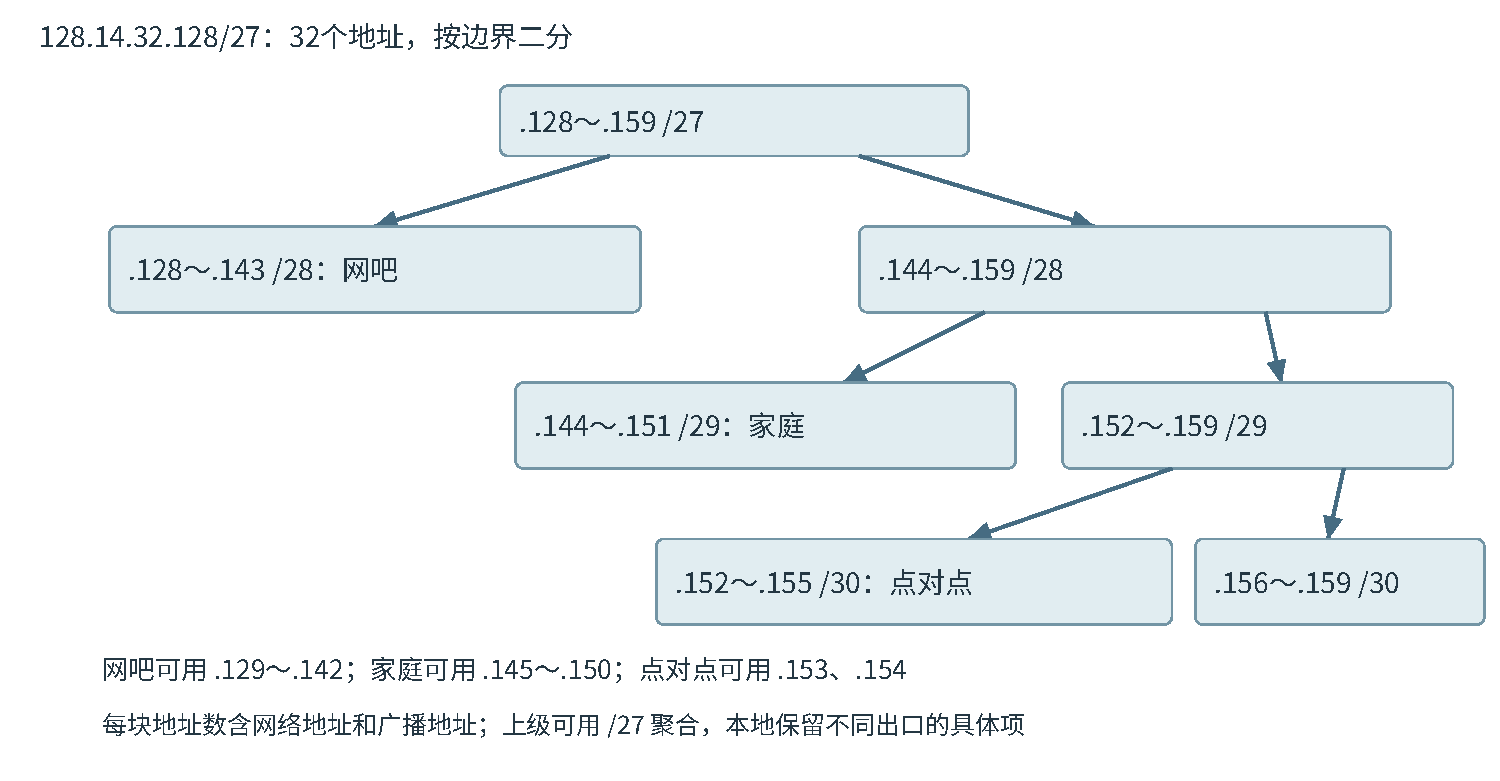
\includegraphics[width=\linewidth,height=108mm,keepaspectratio]{figures/CN_course_vlsm.pdf}
\caption{地址块逐级二分与VLSM对齐}\label{cn-course-vlsm}
\end{figure}

\section{路由聚合与最长前缀匹配}\label{CN04-prefix}

精确聚合须连续、对齐、同出口，汇总块完全覆盖且不额外包含其他地址；等长\(2^s\)块聚合时前缀缩短\(s\)位。允许覆盖空隙时，须保留需要的更具体路由，并检查未分配范围的丢弃或回程环路。

\par\medskip\Needspace{4\baselineskip}\noindent\hypertarget{CN04-E05}{}\label{CN04-E05}\textbf{例 4-5}\par\nobreak\smallskip

某路由表中有转发接口相同的4条路由表项，其目的网络地址分别为 \texttt{35.\allowbreak{}230.\allowbreak{}32.\allowbreak{}0/\allowbreak{}21}、\texttt{35.\allowbreak{}230.\allowbreak{}40.\allowbreak{}0/\allowbreak{}21}、\texttt{35.\allowbreak{}230.\allowbreak{}48.\allowbreak{}0/\allowbreak{}21} 和 \texttt{35.\allowbreak{}230.\allowbreak{}56.\allowbreak{}0/\allowbreak{}21}，将该4条路由聚合后的目的网络地址为（　）。

A. 35.230.0.0/19　B. 35.230.0.0/20

C. 35.230.32.0/19　D. 35.230.32.0/20

查表先选匹配位数最多的前缀，再读取输出接口及下一跳；不同前缀长度间不直接比较度量。\texttt{/\allowbreak{}32}仅匹配一主机，\texttt{/\allowbreak{}0}为无更具体匹配时的默认路由，仍遵守广播、TTL等限制。本地出口与下一跳IP是两个字段。

\par\medskip\Needspace{4\baselineskip}\noindent\hypertarget{CN04-E11}{}\label{CN04-E11}\textbf{例 4-6}\par\nobreak\smallskip

Internet的两个自治系统构成的网络如下图所示。AS1由R1连接两个子网构成；AS2由R2、R3互联并连接三个子网构成。各子网地址、R2的接口名以及R1、R3的部分接口IP地址均在图中标出。

\begin{figure}[H]
\centering
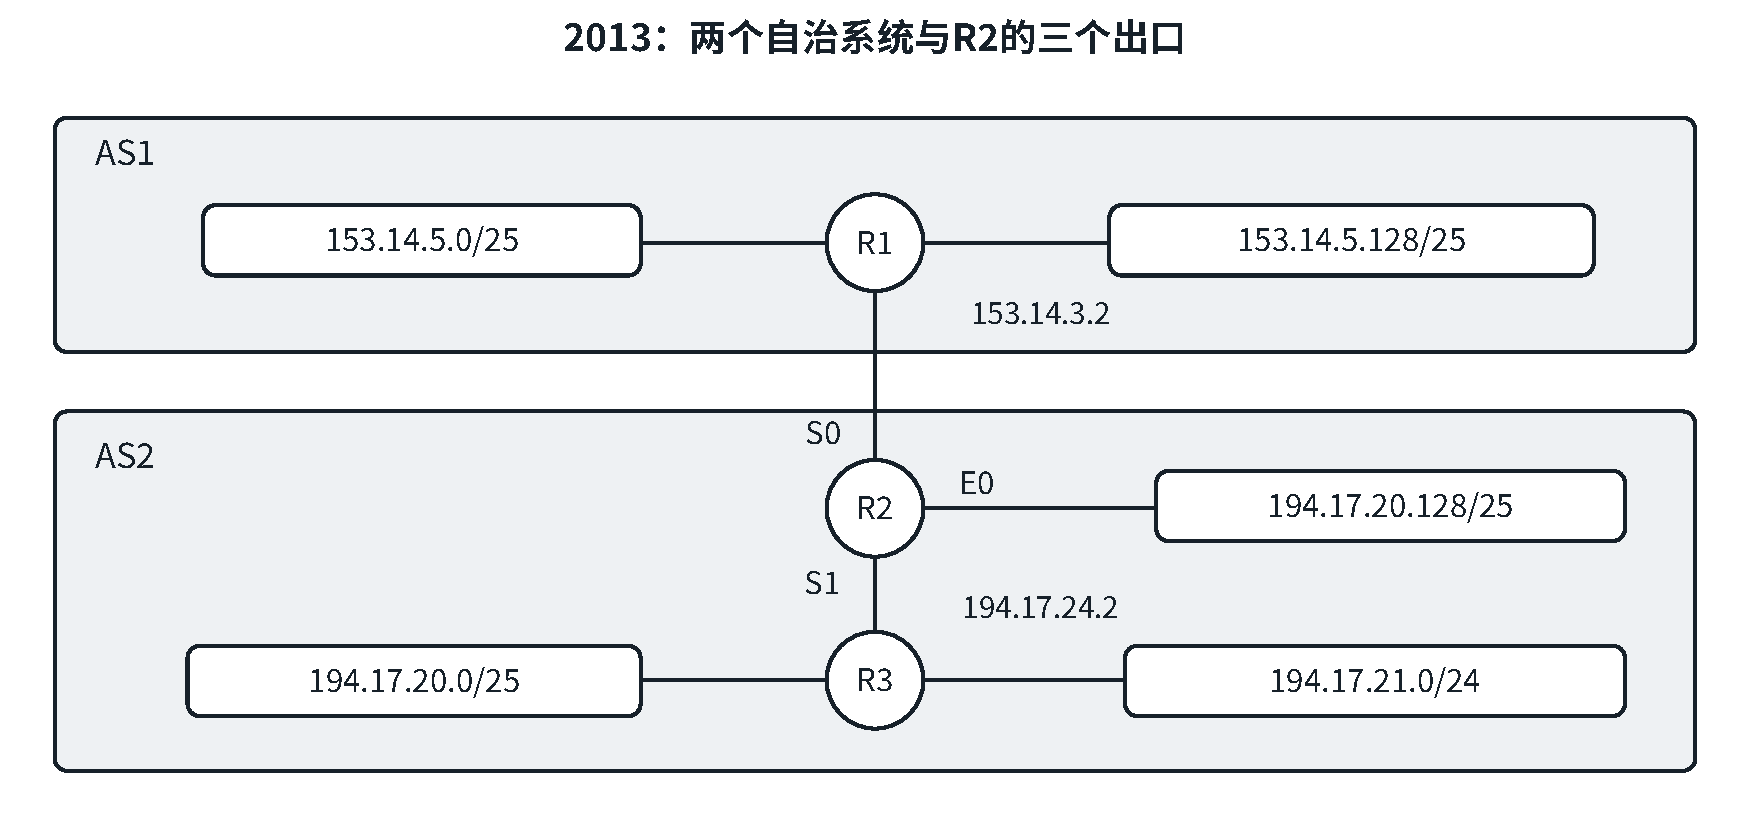
\includegraphics[width=\linewidth,height=108mm,keepaspectratio]{figures/CN22_aggregate_2013.pdf}
\caption{R2经S0到R1、经S1到R3，E0直连194.17.20.128/25}\label{cn-fig-aggregate2013}
\end{figure}

（1）路由表结构为``目的网络、下一跳、接口''。利用路由聚合技术给出R2的路由表，要求包括到达图中所有子网的路由，且路由项尽可能少。

（2）若R2收到目的IP地址为194.17.20.200的IP分组，会通过哪个接口转发？

（3）R1与R2之间利用哪个路由协议交换路由信息？该协议报文封装到哪个协议的数据单元中传输？

\section{ARP、逐跳封装与NAT}\label{CN04-arp-nat}

发送步骤：按掩码和路由判定下一跳\ensuremath{\to}查下一跳IP的ARP缓存\ensuremath{\to}缺项时在本广播域广播ARP请求\ensuremath{\to}目标通常单播回复\ensuremath{\to}以本机出口MAC为源、下一跳MAC为目的封装。

\begin{figure}[H]
\centering
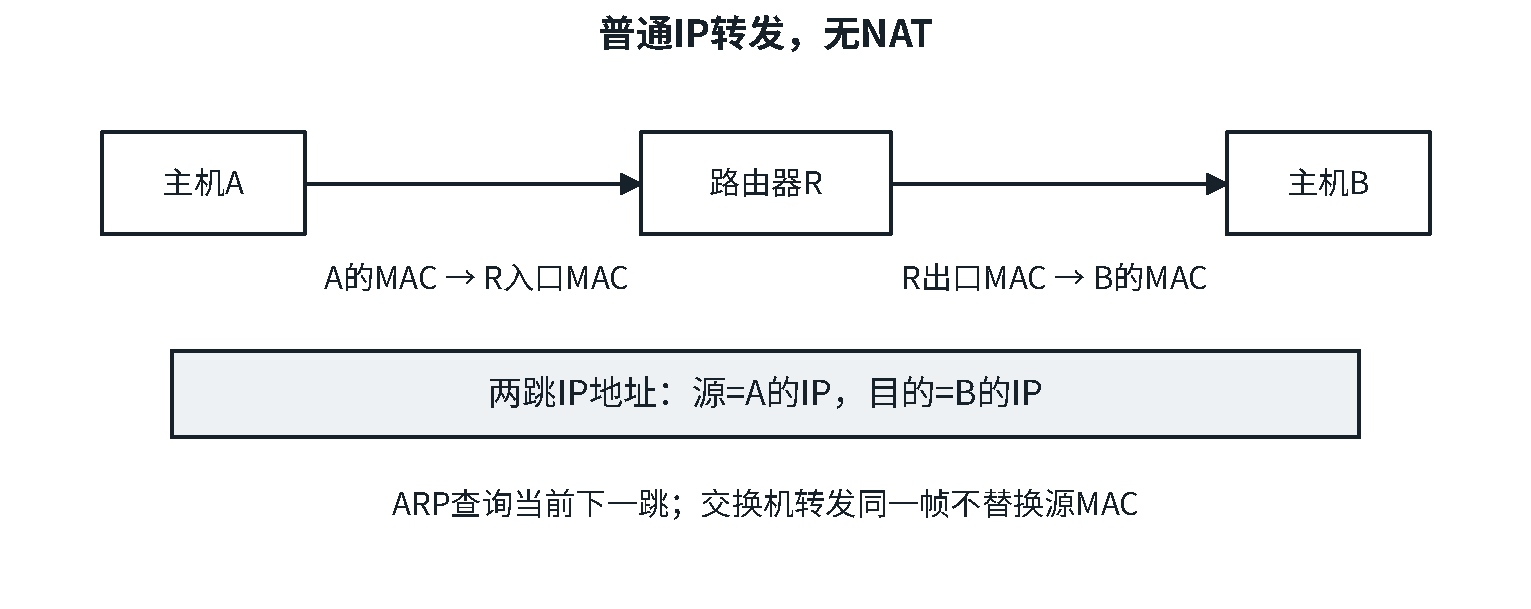
\includegraphics[width=\linewidth,height=108mm,keepaspectratio]{figures/CN08_ip_mac_hops.pdf}
\caption{无NAT时IP两端保持，MAC逐跳重封装}\label{cn-fig-arp}
\end{figure}

目的在本地，ARP查询目的IP；目的在外地，通常查询默认网关或路由指定邻居IP。普通路由器不转发ARP广播。二层交换机转发同一帧时保留源MAC，路由器下一跳重新封装。ARP缓存会老化，代理ARP须有明确条件。

\par\medskip\Needspace{4\baselineskip}\noindent\hypertarget{CN04-E06}{}\label{CN04-E06}\textbf{例 4-7}\par\nobreak\smallskip

某以太网中，甲IP为211.71.136.23，子网掩码255.255.240.0，网关211.71.136.1。若甲向乙211.71.130.25发送IP分组，则（　）。

A. 直接发给乙，帧目的MAC为网关MAC

B. 直接发给乙，帧目的MAC为乙MAC

C. 交网关转发，帧目的MAC为网关MAC

D. 交网关转发，帧目的MAC为乙MAC

NAT在边界维护内部/外部地址映射；NAPT再用端口复用公网IP。普通源NAT出向改源IP，NAPT还可改源端口，回包按映射恢复；远端目的通常保持。IP首部校验随地址改写更新，TCP/UDP伪首部也含IP地址，启用的传输层校验须相应更新。IPv4 UDP全0未启用的情况单独处理。外部主动访问通常需要静态映射、端口转发等机制。

\section{DHCP与ICMP}\label{CN04-control}

DHCP提供IP、掩码、网关、DNS及租期，UDP服务器67、客户端68。初次获取：Discover寻找\ensuremath{\to}Offer提议\ensuremath{\to}Request选择\ensuremath{\to}ACK确认使用；初始Request源\texttt{0.\allowbreak{}0.\allowbreak{}0.\allowbreak{}0}、目的受限广播，申请地址通过Requested IP Address选项携带。续租状态可单播；跨网段可用DHCP中继。

\par\medskip\Needspace{4\baselineskip}\noindent\hypertarget{CN04-E07}{}\label{CN04-E07}\textbf{例 4-8}\par\nobreak\smallskip

一台新接入网络的主机H通过DHCP服务器动态请求IP地址过程中，与DHCP服务器交换DHCP报文的部分过程如下图。封装DHCPREQUEST报文的IP数据报的目的IP地址和源IP地址分别是（　）。

\begin{figure}[H]
\centering
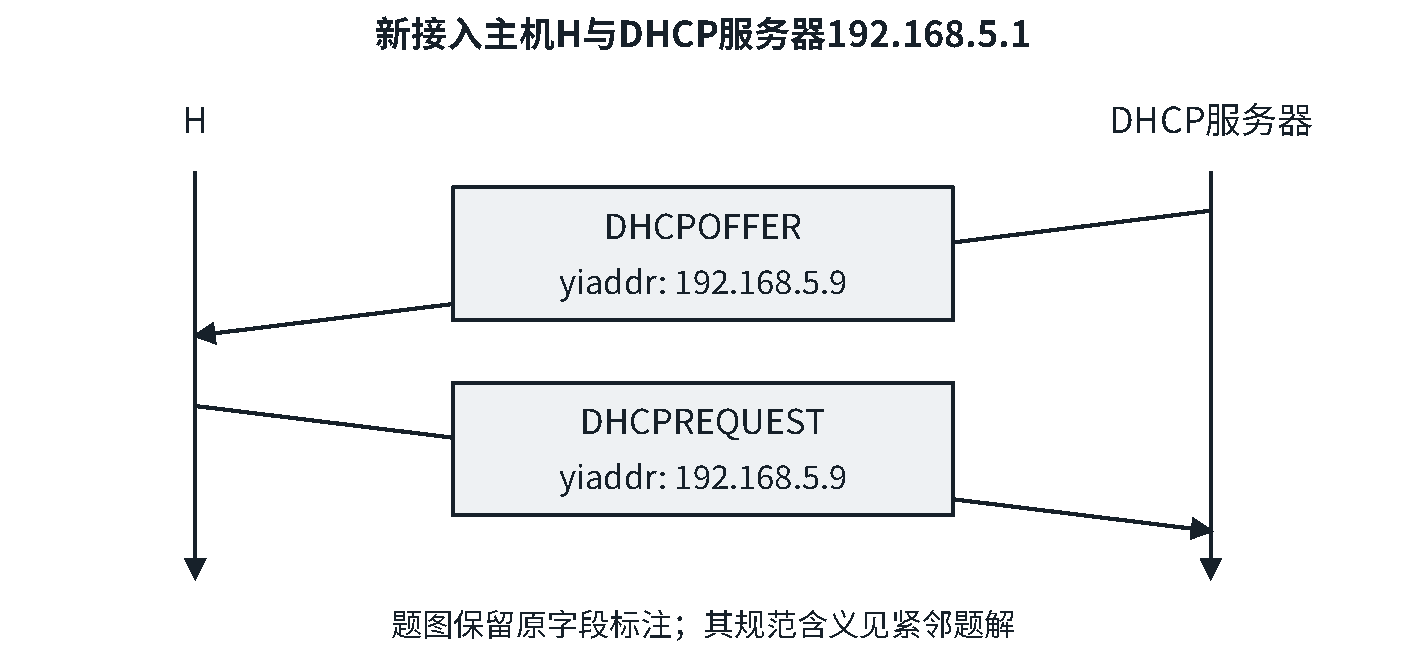
\includegraphics[width=\linewidth,height=108mm,keepaspectratio]{figures/CN13_dhcp_2025.pdf}
\caption{原题的两个报文及字段标记；时间向下}\label{cn-fig-dhcp}
\end{figure}

A. 192.168.5.1，0.0.0.0

B. 192.168.5.1，192.168.5.9

C. 255.255.255.255，0.0.0.0

D. 255.255.255.255，192.168.5.9

ICMP由IP封装，报告目的不可达、时间超过、参数问题等，回送请求/应答用于Ping；错误报告通常含原IP首部及一部分数据，返回原源端，不负责重传。ICMP差错自身、非首片、广播/组播目的和某些特殊源地址通常不再触发ICMP差错。IP首部检验错误通常直接丢弃。

Traceroute逐增TTL，通过沿途超时回复定位，探测可用UDP、ICMP或TCP变体。历史``源点抑制''类型已由RFC 6633废弃；旧题按年代识别，现行拥塞处理使用适用反馈机制。

\par\medskip\Needspace{4\baselineskip}\noindent\hypertarget{CN04-E08}{}\label{CN04-E08}\textbf{例 4-9}\par\nobreak\smallskip

若路由器R因为拥塞丢弃IP分组，则此时R可向发出该IP分组的源主机发送的ICMP报文类型是（　）。

A. 路由重定向　B. 目的不可达　C. 源点抑制　D. 超时

\section{IPv6首部、地址与过渡}\label{CN04-ipv6}

IPv6地址128 bit，8组16位十六进制，单组可省前导0，\texttt{:\allowbreak{}:\allowbreak{}}最多一次，恢复至8组。基本首部固定40 B：版本4 bit、流量类别8 bit、流标签20 bit、有效载荷长度16 bit、下一首部8 bit、跳数限制8 bit、源/目的各128 bit。

\par\smallskip
{\fontsize{9.3}{12}\selectfont\setlength{\tabcolsep}{2.5pt}\setlength{\LTleft}{0pt}\setlength{\LTright}{0pt}
\begin{longtable}{@{}>{\raggedright\arraybackslash}p{\dimexpr0.28990\linewidth-2\tabcolsep\relax}>{\raggedright\arraybackslash}p{\dimexpr0.71010\linewidth-2\tabcolsep\relax}@{}}
\toprule
项目 & IPv6规则 \\

\midrule\endfirsthead\toprule
项目 & IPv6规则 \\

\midrule\endhead\bottomrule\endfoot
长度 & 有效载荷长度计基本首部后的扩展首部和上层数据 \\

扩展 & 下一首部可指扩展首部或上层协议，基本首部无首部校验和 \\

转发与分片 & 路由器不分片，过大时发Packet Too Big；源端按路径MTU调整或加分片扩展首部 \\

邻居与广播 & 无广播；用ICMPv6邻居发现取代ARP \\

地址 & 未指定\texttt{::}，回环\texttt{::1}，链路本地\texttt{fe80::/10}，组播\texttt{ff00::/8} \\

任播 & 多接口共地址，按路由交付其中一个 \\

配置 & 支持无状态自动配置和DHCPv6，接口标识生成不限于MAC \\

\end{longtable}}
\par\smallskip

IPv6地址空间/IPv4地址空间为\(2^{96}\)。双栈同时运行两协议；隧道把一类IP分组封装到另一类IP分组中，内外端点分别解释。流量类别、流标签仅提供分类信息，服务保证还需要资源和机制。

\par\medskip\Needspace{4\baselineskip}\noindent\hypertarget{CN04-E09}{}\label{CN04-E09}\textbf{例 4-10}\par\nobreak\smallskip

下列关于IPv4和IPv6的叙述中，正确的是（　）。

I. IPv6地址空间是IPv4地址空间的96倍

\begin{enumerate}
\def\labelenumi{\Roman{enumi}.}
\setcounter{enumi}{1}
\item
  IPv4首部和IPv6基本首部的长度均可变
\item
  IPv4向IPv6过渡可以采用双协议栈和隧道技术
\item
  IPv6首部的Hop Limit字段等价于IPv4首部的TTL字段
\end{enumerate}

A. 仅I、II　B. 仅I、IV　C. 仅II、III　D. 仅III、IV

\section{RIP、OSPF与BGP}\label{CN04-routing-protocols}

自治系统AS为统一管理和路由策略下的一组网络与路由器。IGP负责AS内部，域间协议交换AS间可达性；AS可含多子网、多出口。

\par\smallskip
\begin{wideblock}
{\fontsize{9.3}{12}\selectfont\setlength{\tabcolsep}{2.5pt}\setlength{\LTleft}{0pt}\setlength{\LTright}{0pt}
\begin{longtable}{@{}>{\raggedright\arraybackslash}p{\dimexpr0.14609\linewidth-2\tabcolsep\relax}>{\raggedright\arraybackslash}p{\dimexpr0.27410\linewidth-2\tabcolsep\relax}>{\raggedright\arraybackslash}p{\dimexpr0.28291\linewidth-2\tabcolsep\relax}>{\raggedright\arraybackslash}p{\dimexpr0.29690\linewidth-2\tabcolsep\relax}@{}}
\toprule
项目 & RIP & OSPF & BGP \\

\midrule\endfirsthead\toprule
项目 & RIP & OSPF & BGP \\

\midrule\endhead\bottomrule\endfoot
方法 & 距离向量，跳数 & 链路状态，SPF & 路径向量，策略 \\

范围 & AS内 & AS内、区域 & AS间，并在AS内传播BGP路由 \\

核心信息 & 到目的的距离 & 本地链路状态，范围内洪泛 & 前缀、AS\_PATH、NEXT\_HOP等属性 \\

承载 & UDP520 & IP协议89 & TCP179 \\

更新 & 通常30 s周期及触发；坏消息慢 & 变化更新、刷新、老化和可靠洪泛 & 会话建立后增量发布/撤销，保活另行 \\

\end{longtable}}
\end{wideblock}
\par\smallskip

RIP最大可达15，16为不可达；教材直连网距离计1，邻居报告加1并改下一跳为邻居。未登记则加入；候选更优则替换；原下一跳就是该邻居时，采用其新距离，即使变差；其他邻居较差通常保留原项。失效判断课件示例180 s。

OSPF区域内同步拓扑，跨区经骨干区域，边界路由器参与多个区域。LSDB为数据库，LSA为通告，五种分组如下。

\par\smallskip
{\fontsize{9.3}{12}\selectfont\setlength{\tabcolsep}{2.5pt}\setlength{\LTleft}{0pt}\setlength{\LTright}{0pt}
\begin{longtable}{@{}>{\raggedright\arraybackslash}p{\dimexpr0.28878\linewidth-2\tabcolsep\relax}>{\raggedright\arraybackslash}p{\dimexpr0.28878\linewidth-2\tabcolsep\relax}>{\raggedright\arraybackslash}p{\dimexpr0.42245\linewidth-2\tabcolsep\relax}@{}}
\toprule
类型 & 分组 & 作用 \\

\midrule\endfirsthead\toprule
类型 & 分组 & 作用 \\

\midrule\endhead\bottomrule\endfoot
1 & Hello & 发现、维持邻居 \\

2 & DD & 数据库摘要，LSA头 \\

3 & LSR & 请求缺失或更新LSA \\

4 & LSU & 发送LSA正文并洪泛 \\

5 & LSAck & 确认收到LSA \\

\end{longtable}}
\par\smallskip

BGP的AS\_PATH用于AS环检测和策略，含本AS号通常拒绝；NEXT\_HOP还需IGP递归求本机出口。eBGP两端属不同AS，iBGP同AS且不必物理直连；完整网状iBGP可由路由反射等机制扩展。OPEN交换会话参数，UPDATE发布/撤销，KEEPALIVE保活，NOTIFICATION报告错误并结束。按题给本地偏好、AS路径等规则选路；属性相同的教材题才进一步比较到出口域内代价。

\par\medskip\Needspace{4\baselineskip}\noindent\hypertarget{CN04-E12}{}\label{CN04-E12}\textbf{例 4-11}\par\nobreak\smallskip

网络空间是继陆海空天之后的``第五疆域''，路由算法与协议是网络核心技术之一。现有互联网中4个自治系统的互连拓扑如下图。AS1运行RIP；AS3内任意两台主机通信经过的路由器不超过15个，AS4内可能超过20个。本题采用下图拓扑：\textbf{R13与R16不直接相连}。

\begin{figure}[H]
\centering
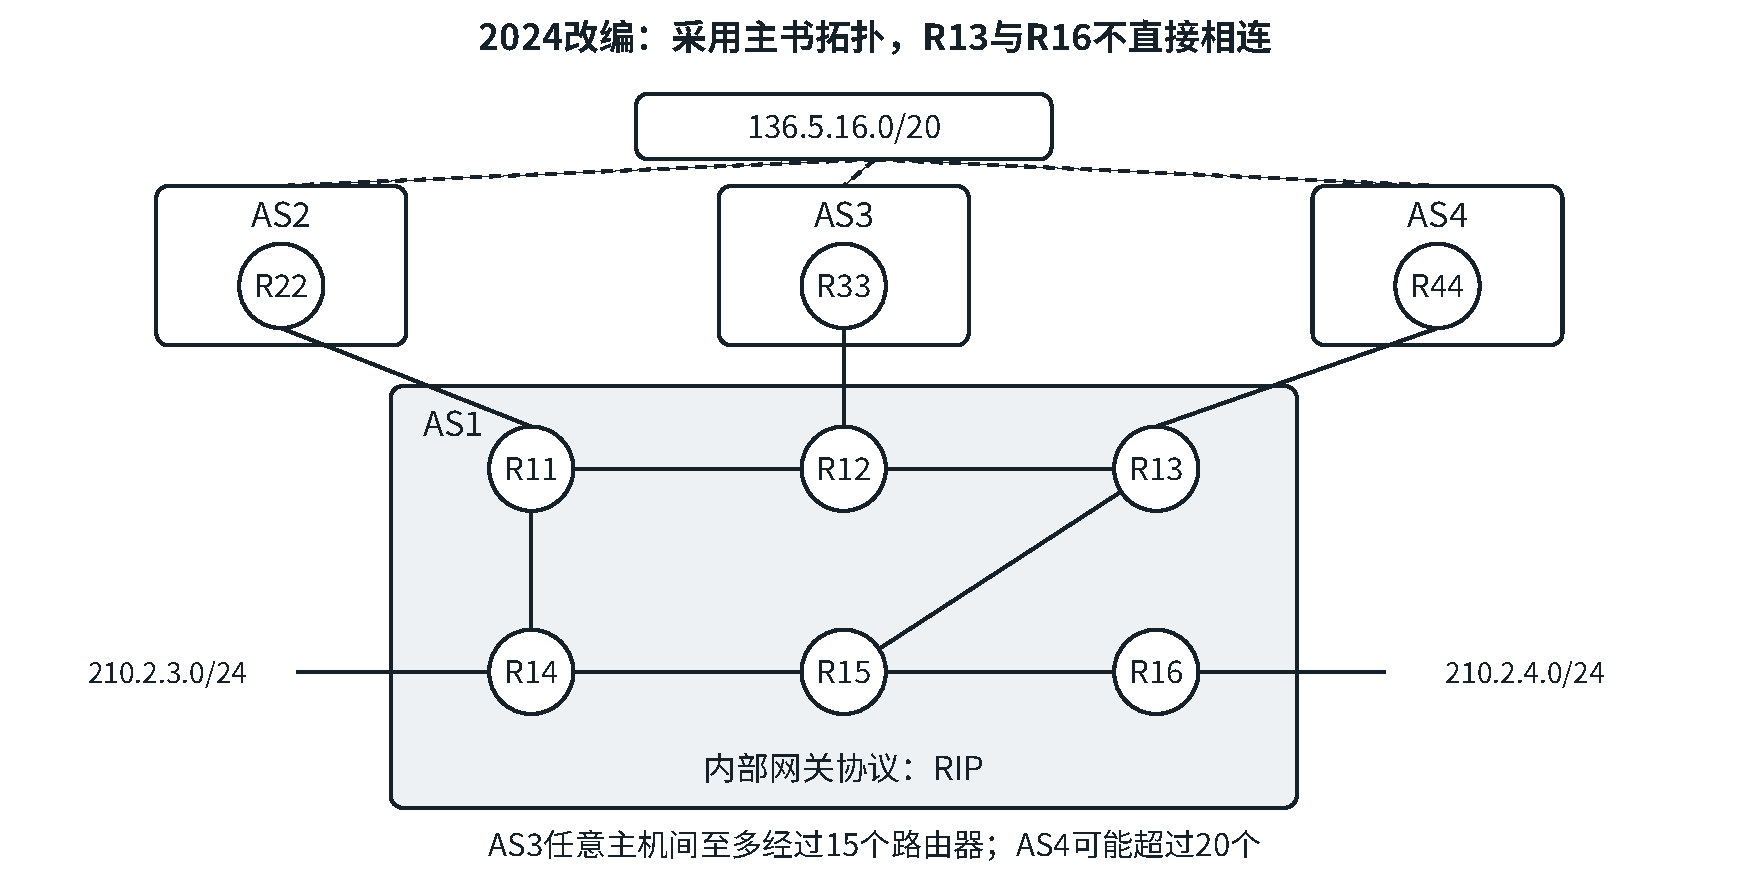
\includegraphics[width=\linewidth,height=108mm,keepaspectratio]{figures/CN23_routing_2024.pdf}
\caption{AS1内仅有R11---R12、R12---R13、R11---R14、R14---R15、R15---R16、R15---R13六条路由器间链路}\label{cn-fig-routing2024}
\end{figure}

（1）若仅有RIP、OSPF可选，AS4应选择哪个内部网关协议？

（2）AS3中的某主机向本AS另一主机发送一个IP分组，为保证正常接收，初始TTL至少应为多少？

（3）AS1的路由器同时启动，立即构建并交换初始距离向量，此后每隔30 s交换一次最新距离向量。从交换初始向量的时刻算起，R11～R16全部获得到达210.2.3.0/24的正确路由至少需多久？全部获得到达210.2.4.0/24的正确路由至少需多久？

（4）R44向R13通告136.5.16.0/20的路由，由哪类BGP会话完成、通过哪种BGP报文通告？R13又通过哪类会话将该可达性信息通告给R14、R15？

（5）R14、R15均收到下表可达性信息。在无策略约束的情况下，更新后两者到136.5.16.0/20的下一跳各是谁？

\par\smallskip
{\fontsize{9.3}{12}\selectfont\setlength{\tabcolsep}{2.5pt}\setlength{\LTleft}{0pt}\setlength{\LTright}{0pt}
\begin{longtable}{@{}>{\raggedright\arraybackslash}p{\dimexpr0.33307\linewidth-2\tabcolsep\relax}>{\raggedright\arraybackslash}p{\dimexpr0.41073\linewidth-2\tabcolsep\relax}>{\raggedright\arraybackslash}p{\dimexpr0.25621\linewidth-2\tabcolsep\relax}@{}}
\toprule
目的网络 & AS路径 & 下一跳 \\

\midrule\endfirsthead\toprule
目的网络 & AS路径 & 下一跳 \\

\midrule\endhead\bottomrule\endfoot
136.5.16.0/20 & AS2、AS8、AS19 & R11 \\

136.5.16.0/20 & AS3、AS7、AS11、AS19 & R12 \\

136.5.16.0/20 & AS4、AS10、AS19 & R13 \\

\end{longtable}}
\par\smallskip

\section{组播与移动IP}\label{CN04-multicast-mobility}

IPv4组播\texttt{224.\allowbreak{}0.\allowbreak{}0.\allowbreak{}0/\allowbreak{}4}表示接收者组，公共路径只传一份，在分叉接口复制。以太网组播MAC由\texttt{01:\allowbreak{}00:\allowbreak{}5E}和IP低23位映射，32个IP组播地址可映射同一MAC，上层仍须检查组成员。IGMP管理主机与相邻路由器的本地成员关系，跨网转发树由组播路由协议建立。

移动IPv4保留归属地址，用转交地址表示当前位置，向归属代理注册绑定。传统三角路由：对端\ensuremath{\to}归属网络\ensuremath{\to}归属代理隧道送转交地址\ensuremath{\to}解封装交移动节点；内层目的为归属地址，外层目的为转交地址。基础模型中移动节点可直接发给对端，源地址过滤等条件下可用反向隧道。

\section{路由器结构与综合计算}\label{CN04-router}

输入端口接收、链路检查、查表；交换结构把分组送到输出端；输出端排队、封装、发送；路由处理器维护控制协议和表。交换结构可用内存、总线或互联网络，容量和并行性各异。多个输入争同一输出会排队；输入队首等待忙出口可阻挡后续去空闲出口的分组，称队首阻塞。

普通IPv4转发顺序：接收帧并检查\ensuremath{\to}取出IP\ensuremath{\to}若目的本机按协议上交\ensuremath{\to}否则检查TTL、最长前缀选出口和下一跳\ensuremath{\to}按MTU/DF处理\ensuremath{\to}解析下一跳地址\ensuremath{\to}出口排队并重封装。直通等特殊实现的启动时间按题设。

\par\medskip\Needspace{4\baselineskip}\noindent\hypertarget{CN04-E10}{}\label{CN04-E10}\textbf{例 4-12}\par\nobreak\smallskip

某公司的网络如下图所示。IP地址空间192.168.1.0/24被均分给销售部和技术部两个子网，并已分别为部分主机和路由器接口分配了IP地址。销售部子网的MTU=1500 B，技术部子网的MTU=800 B。

\begin{figure}[H]
\centering
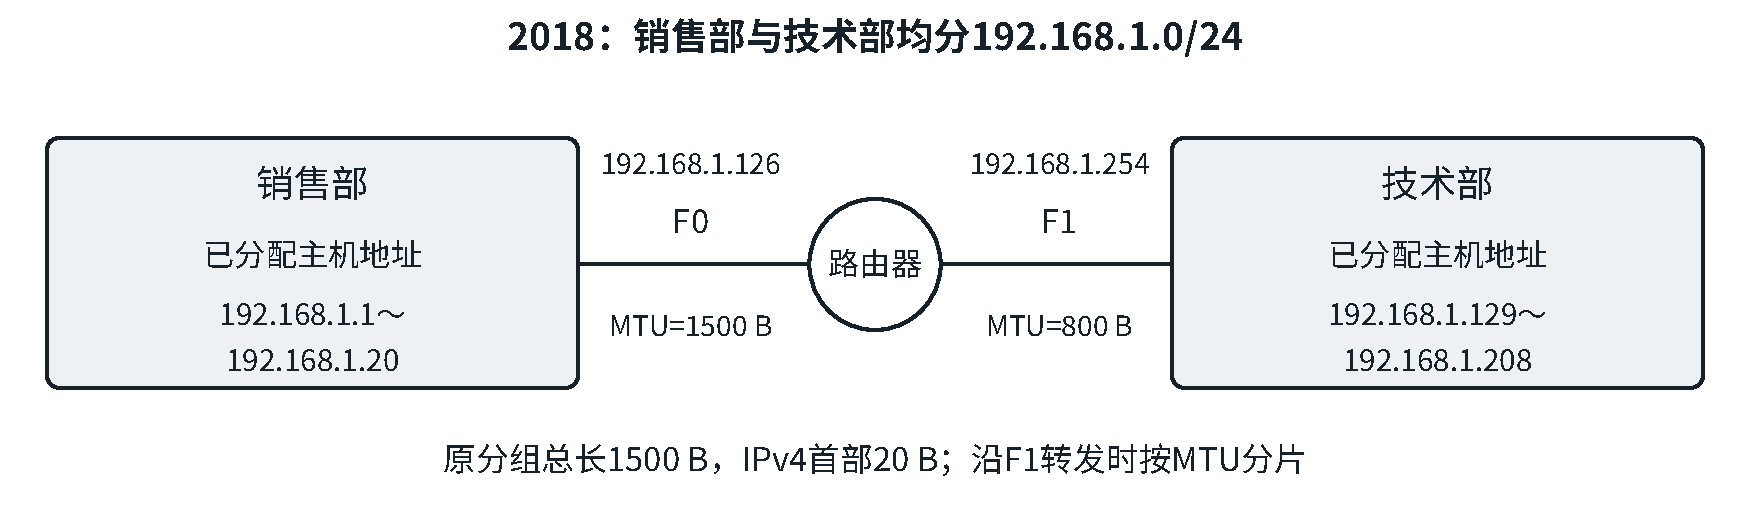
\includegraphics[width=\linewidth,height=108mm,keepaspectratio]{figures/CN21_subnet_fragment_2018.pdf}
\caption{销售部已分配192.168.1.1～20，技术部已分配192.168.1.129～208；F0为.126，F1为.254}\label{cn-fig-subnet2018}
\end{figure}

（1）销售部子网的广播地址是什么？技术部子网的子网地址是什么？若每个主机仅分配一个IP地址，则技术部子网还可以连接多少台主机？

（2）主机192.168.1.1向主机192.168.1.208发送一个总长度为1500 B、首部长度为20 B的IP分组。路由器通过F1转发时进行分片，且尽可能分为最大片。一个最大IP分片封装数据的字节数是多少？至少需要几个分片？每个分片的片偏移量是多少？

\par\medskip\Needspace{4\baselineskip}\noindent\hypertarget{CN04-E13}{}\label{CN04-E13}\textbf{例 4-13}\par\nobreak\smallskip

某公司工程部长期驻扎偏远山区，租用天通一号卫星通信链路连接工程部R1和总部R2，网络如下图。S1、S2为千兆以太网交换机；TR1、TR2是卫星地面收发设备，实现全双工调制解调。卫星轨道高度36000 km，电磁波传播速度300000 km/s；卫星链路为R1、R2提供对称全双工信道，每方向数据传输速率200 kb/s。

\begin{figure}[H]
\centering
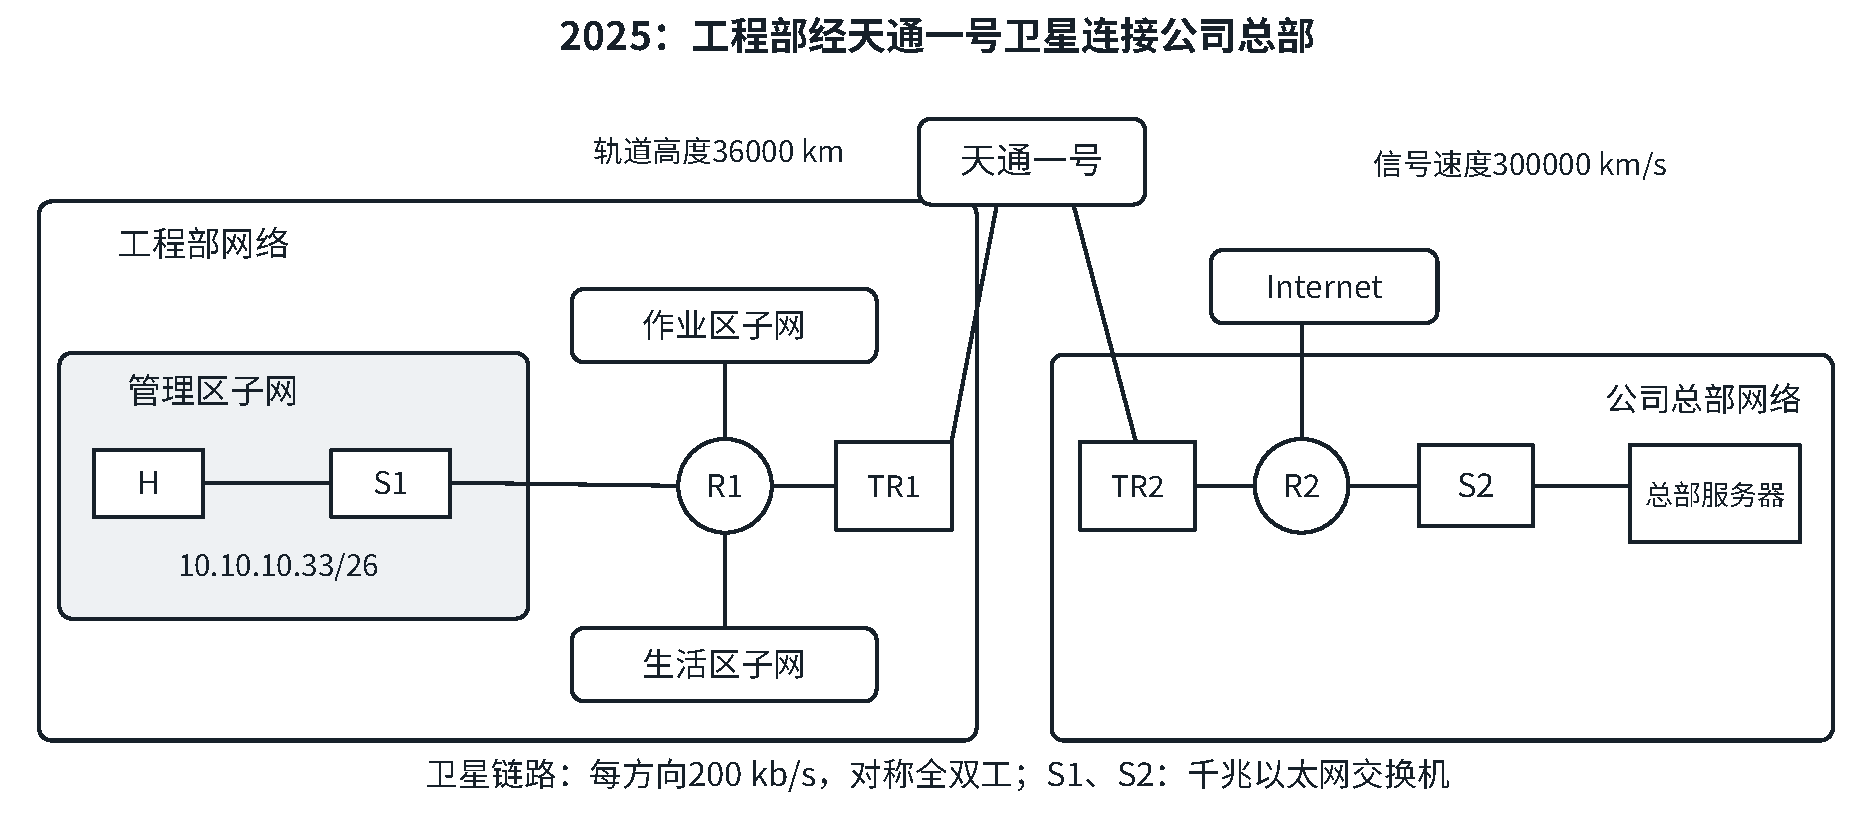
\includegraphics[width=\linewidth,height=108mm,keepaspectratio]{figures/CN24_satellite_2025.pdf}
\caption{H配置10.10.10.33/26并位于管理区；工程部还有作业区、生活区两个子网}\label{cn-fig-satellite2025}
\end{figure}

（1）忽略卫星中继及TR1、TR2调制解调开销，卫星链路单向传播时延是多少？H向总部服务器传输数据可达到的最大吞吐量是多少？忽略各层首部开销与以太网内传播时延，上传4000 B工程进度报告文件至少需要多久？

（2）用GBN为卫星链路设计单向可靠的数据链路层协议SLP，支持R1向R2发送数据。SLP数据帧长1500 B，忽略ACK帧长度；要求单向信道利用率不低于80\%，发送窗口至少为多少？帧序号字段至少需要几位？

（3）总部分配10.10.10.0/24给工程部，需划给三个子网：生活区可分配地址不少于120个，作业区、管理区分别不少于60个，H的地址配置正确。作业区、管理区、生活区的子网地址分别是什么？请用CIDR表示。
